\documentclass{article}
\usepackage{xeCJK}
\setCJKmainfont{FandolSong}
\setCJKmonofont{Noto Sans Mono CJK SC}
\usepackage{amsmath}
\usepackage{amsthm}
\usepackage{amssymb}
\usepackage[noend]{algpseudocode}
\usepackage[margin=1in]{geometry}
\usepackage{float}
\usepackage{hyperref}
\setlength{\parindent}{0pt}
\renewcommand{\thesection}{\arabic{section}}
\newcommand{\problem}{\refstepcounter{section}\section*{Problem \thesection}}
\renewcommand{\thesubsection}{(\alph{subsection})}
\newcommand{\subproblem}[1][]{\refstepcounter{subsection}\paragraph{\thesubsection{}#1}\hspace{0pt}}
\newcommand{\tightsubproblem}[1][]{\refstepcounter{subsection}\textbf{\thesubsection#1\hspace{2ex}}}
\newcommand{\ta}[1]{\textsc{#1}}
\newcommand{\admit}{\hfill$\square$}
\newtheorem{lem}{Lemma}
\newtheorem{thm}{Thm}[section]
\newtheorem{co}{Co}[thm]
\algrenewcommand\algorithmiccomment[1]{\hfill// #1}
\renewcommand\qedsymbol{$\blacksquare$}
\newenvironment{algo}[3][1]{

\vspace{1em}
\begin{minipage}{\linewidth}
\ta{#2}($#3$)
\begin{algorithmic}[#1]
}{\end{algorithmic}\end{minipage}}

\author{221900006 耿天成}
\date{\today}
\usepackage{tikz}
\usetikzlibrary{arrows.meta, backgrounds, quotes}
\renewcommand{\thefootnote}{\roman{footnote}}

\title{ALG Problem Set 11}
\tikzset{
    gnode/.style={circle,draw=orange,fill=orange!20,minimum size=15pt,inner sep=0pt},
    bnode/.style={fill=black,text=white,font=\boldmath},
    tt/.style={fill=none,draw=none,text=black,inner sep=0pt},
    emph/.style={draw, gray!50, line width=5pt},
    graph/.style={
        every node/.style=gnode,
        every edge/.style={draw,thick},
    },
    dgraph/.style={
        every node/.style=gnode,
        every edge/.style={draw,->,>=Stealth},
    }
}
\begin{document}
\maketitle

\problem %1
Let $f(n)$ be the minimum number of steps to produce $n$.
Suppose in an optimal operation sequence to produce $n$, it produces $\lfloor n/2\rfloor-k$ before the last {\it double} for some $k\ge 0$.
\begin{align}
f(n)&=f(\lfloor n/2\rfloor-k)+1+n-2(\lfloor n/2\rfloor-k)\notag\\
    &=f(\lfloor n/2\rfloor-k)+1+n\text{ mod } 2+2k
\end{align}
(If the sequence only contains $+1$, replace the first $+1$ with $\times 2$). \\
We can produce $\lfloor n/2\rfloor$ by increasing $k$ times after obtaining $\lfloor n/2\rfloor-k$.
\begin{equation}f(\lfloor n/2\rfloor)\le f(\lfloor n/2\rfloor-k)+k\end{equation}
Together, (1) and (2) imply that
$$f(n)\ge f(\lfloor n/2\rfloor)+1+n\text{ mod } 2+k$$
\begin{equation}
f(n)\ge f(\lfloor n/2\rfloor)+1+n\text{ mod } 2
\end{equation}
But $n$ can be obtained by doubling $\lfloor n/2\rfloor$, and increasing it if $n$ is odd.
\begin{equation}
f(n)\le f(\lfloor n/2\rfloor) +1+n\text{ mod }2
\end{equation}
Therefore, $f(n)=f(\lfloor n/2\rfloor) +1+n\text{ mod }2$. Combined with $f(1)=0$, we can compute any $f(n)$ in $O(\lg n)$ time.
\begin{algorithmic}[1]
\State $step=0$
\While{$n>1$}
    \If{$step$ mod $2=0$}
        \State $step=step+1$
    \Else
        \State $step=step+2$
    \EndIf
    \State $n=n/2$
\EndWhile
\State \Return $step$
\end{algorithmic}
\problem %2
\subproblem %a
Assume to the contrary that there is no codeword of length 1. Then the root of the Huffman tree cannot have a leaf as a direct child. Suppose one child of the root has children $A, B$, and the other has children $C, D$. Without loss of generality, assume $w(A)\le w(B), w(C)\le w(D)$, and the merge of $A$ and $B$ happened first. We have $w(A)\le w(B)\le w(C)\le w(D)\le w(A)+w(B)$. Some character occurs more than $2/5$, so $w(D)>2/5$. Then $w(C)\ge w(B)\ge(w(A)+w(B))/2>1/5$. $1=w(A)+w(B)+w(C)+w(D)>2/5+1/5+2/5=1$, contradictory. Therefore, there is a codeword of length 1.
\subproblem %b
Assume to the contrary that there is a codeword $A$ of length 1. Since all characters occur less than 1/3, there are at least 4 characters. Suppose $A$ is merged with $X$, and $X$ is merged by $B$ and $C$, $w(B)\le w(C)$. Then we have $w(B)\le w(C)\le w(A)<1/3$. $1=w(A)+w(B)+w(C)>1/3\times3=1$, contradictory. Therefore, there is no codeword of length 1.
\section*{Bonus Problem}\setcounter{subsection}{0}
\subproblem %a
Let $w_i=\frac{|S_i|}{c(S_i)}$. Choose the set $X$ with the largest $w$, remove elements in $X$ from other $S_i$, and recurse.
\begin{algorithmic}[1]
\For{$i=1$ to $k$}
    \State $w[i]=|S_i|/c(S_i)$
\EndFor
\While{$U\neq\emptyset$}
    \State Select set $X\in\mathcal{S}$ that maximizes $w[i]$
    \State $A=A\cup \{X\}$
    \For{each $j\in X\cup U$}
        \State $U = U - \{j\}$
        \For{$k : j \in S_k$}
            \State Decrease $|S_k|$ and update $w[i]$.
        \EndFor
    \EndFor
\EndWhile
\State \Return $A$
\end{algorithmic}
\paragraph{Running time} The number of iterations of the loop on lines 3-9 is bounded by $\min\{n,k\}$.
And the loop on lines 6-9 takes amortized $O(\sum_{i=1}^k |S_i|)$. So the total running time of the algorithm is $O(k\min\{n, k\}+\sum_{i=1}^k |S_i|)$, which is polynomial with respect to the input length.
\paragraph{Approximation ratio} CLRS Problem 35-3 asks us to prove that, let $d$ be the maximum of $|S_i|$, the approximation ratio is $H(d)=\sum_{i=1}^d 1/i$. But we will prove a loose ratio of $H(n)$, and thus the algorithm gives a solution with cost $O({\it OPT}\cdot\ln n)$.
\begin{proof}
Induction on $n$. When $n=1$, $A=\{S_1\}={\it OPT}$.\\
Let $A'$ be the algorithm's solution on subproblem $U-X, \mathcal{S}-\{X\}$, and the optimal cost is $\it OPT'$. By the induction hypothesis, $c(A')\le {\it OPT'}\cdot H(n-|X|)$.
We need to show that $c(A) \le \it{OPT}\cdot H(n)$. Since $X$ can cover the most elements per unit cost, ${\it OPT}\ge n/w(X)$. And $\it OPT\ge OPT'$.
\begin{flalign*}
& c(A') \le OPT'\cdot H(n-|X|) & \\
\implies & c(A')+c(X)\le {\it OPT}\cdot H(n) - {\it OPT}\left(\frac{1}{n-|X|+1}+\cdots +\frac1n\right)+c(X) \\
\implies & c(A) \le {\it OPT}\cdot H(n) + c(X)- \frac{n}{|X|/c(X)}\frac{|X|}{n} \\
\implies & c(A)\le {\it OPT}\cdot H(n)
\end{flalign*}
\end{proof}
\subproblem %b
The construction is from Wikipedia \cite{wikipedia:set-cover}.
There is an example in which the greedy algorithm achieves an approximation ratio $\ge \lg(n)/2$. $U$ consists of $n=2^{k+1}-2$ elements. $\mathcal{S}=\{R_1,\cdots R_k, T_1, T_2\}$, where $R_i = \{2^i-1, 2^i, \cdots, 2^{i+1}-2\}, T_1=\{2m+1\mid 2m+1\le n\}, T_2=\{2m\mid 2m\le n\}$. All $c(S)=1$. The algorithm will choose all $R_i$ with cost $k$, the optimal solution is $\{T_1, T_2\}$ with cost 2.
\problem %3
\subproblem %a
The following figures show the situation before and after each iteration of the while loop.
$dist$ values appear within the vertices, and shaded edges indicate $parent$. Black vertices are in the set $R$.
\begin{center}
\input{tikz/dij1} 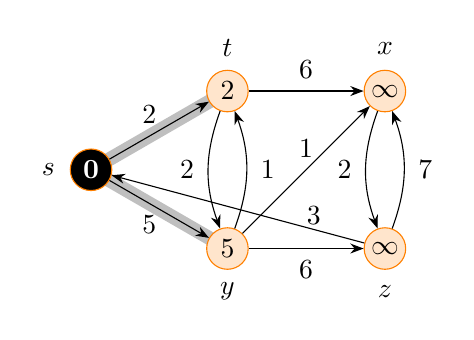
\begin{tikzpicture}[dgraph]
\def\a{1}
\node["$s$" {left},bnode]  (s) at ({-\a*sqrt(3)},0) {$0$};
\node["$t$" {above}] (t) at (0,\a) {$2$};
\node["$x$" {above}] (x) at ({\a*2},\a) {$\infty$};
\node["$y$" {below}] (y) at (0,-\a) {$5$};
\node["$z$" {below}] (z) at ({\a*2},-\a) {$\infty$};
\path
    (t) edge node[tt,above] {$6$} (x)
    (t) edge[bend right=20] node[tt,left] {$2$}(y)
    (x) edge[bend right=20] node[tt,left] {$2$}(z)
    (y) edge[bend right=20] node[tt,right] {$1$} (t)
    (y) edge node[tt,above] {$1$} (x)
    (y) edge node[tt,below] {$6$} (z)
    (z) edge[bend right=20] node[tt,right] {$7$} (x)
    (z) edge node[tt,yshift=5pt,pos=0.2] {$3$} (s)
    (s) edge node[tt,above,pos=0.4] {$2$} (t)
    (s) edge node[tt,below,pos=0.4] {$5$} (y)
;
\scoped[on background layer]{
    \draw[emph] (s.center) -- (t.center);
    \draw[emph] (s.center) -- (y.center);
}
\end{tikzpicture} \input{tikz/dij3}\\
\input{tikz/dij4} 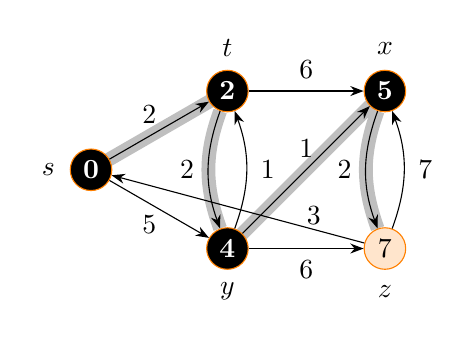
\begin{tikzpicture}[dgraph]
\def\a{1}
\node["$s$" {left},bnode]  (s) at ({-\a*sqrt(3)},0) {$0$};
\node["$t$" {above},bnode] (t) at (0,\a) {$2$};
\node["$x$" {above},bnode] (x) at ({\a*2},\a) {$5$};
\node["$y$" {below},bnode] (y) at (0,-\a) {$4$};
\node["$z$" {below}] (z) at ({\a*2},-\a) {$7$};
\path
    (t) edge node[tt,above] {$6$} (x)
    (t) edge[bend right=20] node[tt,left] {$2$}(y)
    (x) edge[bend right=20] node[tt,left] {$2$}(z)
    (y) edge[bend right=20] node[tt,right] {$1$} (t)
    (y) edge node[tt,above] {$1$} (x)
    (y) edge node[tt,below] {$6$} (z)
    (z) edge[bend right=20] node[tt,right] {$7$} (x)
    (z) edge node[tt,yshift=5pt,pos=0.2] {$3$} (s)
    (s) edge node[tt,above,pos=0.4] {$2$} (t)
    (s) edge node[tt,below,pos=0.4] {$5$} (y)
;
\scoped[on background layer]{
    \draw[emph] (s.center) -- (t.center);
    \path (t) edge[-,emph,bend right=20] (y);
    \draw[emph] (y.center) -- (x.center);
    \path (x) edge[-,emph,bend right=20] (z);
}
\end{tikzpicture} \input{tikz/dij6}
\end{center}
\subproblem %b
The following figures show the situation before and after each pass. $dist$ values appear within the vertices, and shaded edges indicate $parent$.
\begin{center}
\input{tikz/bel1} 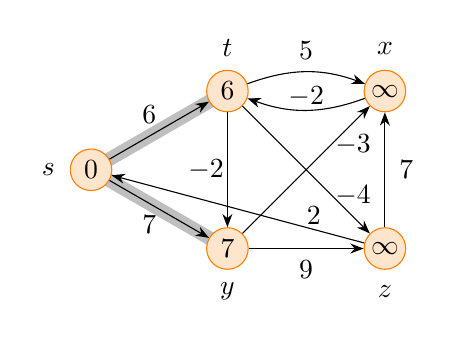
\begin{tikzpicture}[dgraph]
\def\a{1}
\node["$s$" {left}]  (s) at ({-\a*sqrt(3)},0) {$0$};
\node["$t$" {above}] (t) at (0,\a) {$6$};
\node["$x$" {above}] (x) at ({\a*2},\a) {$\infty$};
\node["$y$" {below}] (y) at (0,-\a) {$7$};
\node["$z$" {below}] (z) at ({\a*2},-\a) {$\infty$};
\path
    (t) edge[bend left=20] node[tt,above] {$5$} (x)
    (t) edge node[tt,left] {$-2$}(y)
    (t) edge node[tt,right,pos=0.7] {$-4$} (z)
    (x) edge[bend left=20] node[tt,yshift=5pt] {$-2$} (t)
    (y) edge node[tt,right,pos=0.7] {$-3$} (x)
    (y) edge node[tt,below] {$9$} (z)
    (z) edge node[tt,right] {$7$} (x)
    (z) edge node[tt,yshift=5pt,pos=0.2] {$2$} (s)
    (s) edge node[tt,above,pos=0.4] {$6$} (t)
    (s) edge node[tt,below,pos=0.4] {$7$} (y)
;
\scoped[on background layer]{
    \draw[emph] (s.center) -- (t.center);
    \draw[emph] (s.center) -- (y.center);
}
\end{tikzpicture} \input{tikz/bel3} \\
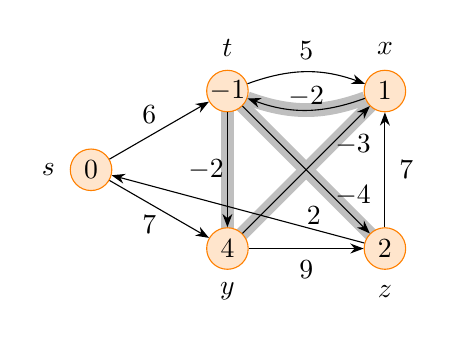
\begin{tikzpicture}[dgraph]
\def\a{1}
\node["$s$" {left}]  (s) at ({-\a*sqrt(3)},0) {$0$};
\node["$t$" {above}] (t) at (0,\a) {$-1$};
\node["$x$" {above}] (x) at ({\a*2},\a) {$1$};
\node["$y$" {below}] (y) at (0,-\a) {$4$};
\node["$z$" {below}] (z) at ({\a*2},-\a) {$2$};
\path
    (t) edge[bend left=20] node[tt,above] {$5$} (x)
    (t) edge node[tt,left] {$-2$}(y)
    (t) edge node[tt,right,pos=0.7] {$-4$} (z)
    (x) edge[bend left=20] node[tt,yshift=5pt] {$-2$} (t)
    (y) edge node[tt,right,pos=0.7] {$-3$} (x)
    (y) edge node[tt,below] {$9$} (z)
    (z) edge node[tt,right] {$7$} (x)
    (z) edge node[tt,yshift=5pt,pos=0.2] {$2$} (s)
    (s) edge node[tt,above,pos=0.4] {$6$} (t)
    (s) edge node[tt,below,pos=0.4] {$7$} (y)
;
\scoped[on background layer]{
    \draw (x) edge[-,emph,bend left=20] (t);
    \draw[emph] (t.center) -- (y.center);
    \draw[emph] (t.center) -- (z.center);
    \draw[emph] (x.center) -- (y.center);
}
\end{tikzpicture} \input{tikz/bel5}
\end{center}
\subproblem %c
The MST of the following graph is $\{(s, x), (x, y)\}$, but the shortest-path tree rooted at $s$ is $\{(s, x), (s, y)\}$.
\begin{center}
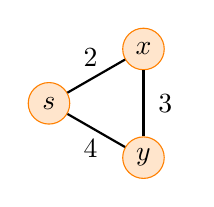
\begin{tikzpicture}[graph]
    \node (s) at (0,0) {$s$};
    \node (x) at (1.2,0.69) {$x$};
    \node (y) at (1.2,-0.69) {$y$};
    \path (s) edge node[tt, above, pos=0.4] {2} (x)
          (x) edge node[tt, right] {3} (y)
          (s) edge node[tt, below, pos=0.4] {4} (y)
    ;
\end{tikzpicture}
\end{center}
No, the 2 trees cannot be completely disjoint. \begin{proof}
We show that the 2 trees share some light cross edge of cut $C=(\{S\},V-\{S\})$.
First, assume that all light cross edge of $C$ is not in $T$. Suppose $(s, u)$ is a light cross edge of $C$, then the simple path between $s$ and $u$ on $T$ contains an edge $(s, v)$. Since $T-\{(s, v)\}\cup\{(s, u)\}$ is a spanning tree of $G$, we have $w(s, u)\ge w(s, v)$, which contradicts that $(s, v)$ is not a light cross edge of $C$. Therefore, $T$ contains some light cross edge $(s, u)$ of $C$.
Then, assume $(s, u)\notin T'$, the simple path from $s$ to $u$ on $T'$ contains an edge $(s, v)$. We have $\delta(s,u)=w(s,v)+\delta(u,v)>w(s,v)\ge w(s,u)$, which contradicts that $\delta(s, u)\le w(s,u)$. Therefore, $T$ and $T'$ both contain $(s, u)$.
\end{proof}
Remark: It is necessary to assume positive weights. If we assume non-negative weights, the following graph has a completely disjoint MST (green) and shortest-path tree (red).
\begin{center}
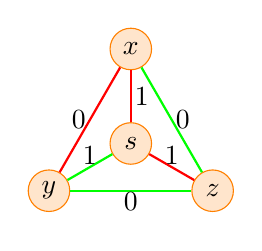
\begin{tikzpicture}[graph]
    \node (s) at (0,0) {$s$};
    \node (x) at (90:1.2) {$x$};
    \node (y) at (210:1.2) {$y$};
    \node (z) at (-30:1.2) {$z$};
    \path
        (s) edge[draw=red] node[tt,xshift=4pt] {1} (x)
        (x) edge[draw=red] node[tt,xshift=-4pt] {0} (y)
        (s) edge[draw=green] node[tt,yshift=4pt] {1} (y)
        (x) edge[draw=green] node[tt,xshift=4pt] {0} (z)
        (y) edge[draw=green] node[tt,yshift=-4pt] {0} (z)
        (s) edge[draw=red] node[tt,yshift=4pt] {1} (z)
    ;
\end{tikzpicture}
\end{center}
\problem %4
\newcommand{\To}[1]{\stackrel{#1}{\leadsto}}
We want to maximize
\begin{equation*}
\prod_{(u, v)\in p} r(u, v)\mid u\To{p}v
\end{equation*}
That is to minimize
\begin{equation*}
\sum_{(u, v)\in p} -\lg(r(u, v))\mid u\To{p}v
\end{equation*}
Since $-\lg(r)\ge 0$, the problem is transformed to a non-negative weight shortest path problem, which can be solved by Dijkstra's algorithm. (In the real world, instead of computing $\lg$, we can modify the \ta{Initialize-Single-Source}, \ta{Relax} procedure and change the min-priority queue to a max-priority queue. We will show how to modify Dijkstra in the next problem 5. The difference is, besides floating point error\footnote{Briefly show the error is acceptable using IEEE 754 format (base 2). Suppose normal floating point number $0<r<1$ is represented as $r=c\times 2^{-q}$, $1 \le c < 2$ is a $p$ bit precision, and $0 < q < 2^e$ is an $e$ bit exponent.\\
Since $-\lg(r)$ has decreasing derivative (absolute value), we study when $r$ is small, where $c$ is close to 1.\\
Let $c_1 = 1, c_2 = 1+2^{-{p}}$. $-\lg(r_1)=q, -\lg(r_2)=q-\lg(1+2^{-p})\approx q-2^{-p}$.
For an $1+e+p$ bit float number $r$, $\lg(r)$ needs $e+p$ bit precision. So if we use \texttt{float}(1+8+23) for $r$ and \texttt{double}(1+11+52) for $-\lg r$, the error will be acceptable.} whether we need to prove the correctness. The $\lg$ hack reduces the problem to the shortest path problem, and nothing is left to prove, while in the next problem, there's no direct transformation. So we modify Dijkstra's algorithm, and only provide a proof schema.)

For {\boldmath $r=0$}, let $-\lg(0)=\infty$, then Dijkstra's algorithm on $(G,(-\lg)\circ r,s)$ will ignore the $\infty$ weight edges since $v.d > u.d + \infty$ never holds.
If $t.\pi\neq\it NIL$, we are done.
If $t.\pi=\it NIL$, there is no path from $s$ to $t$ that does not traverse an edge with reliability 0. Run \ta{BFS}$(G,s)$ to find a path from $s$ to $t$.\\
\ta{Path} is modified from \ta{Print-Path} in Section 22.2.\\[1em]
\ta{Path}$(s,t)$
\begin{algorithmic}[1]
\If{$s=t$}
\State \Return $\left<s\right>$
\EndIf
\If{$t.\pi=\it NIL$}
\State \Return {\it NIL}
\EndIf
\State \Return $\ta{Path}(s, t.\pi)+\left<t\right>$
\end{algorithmic}\vspace{1em}
\ta{MostReliablePath}$(G,r,s,t)$
\begin{algorithmic}[1]
\State \ta{Dijkstra}$(G, (-\lg)\circ r, s)$
\State $path=\ta{Path}(s, t)$
\If{$path\neq\it NIL$}
\State \Return $path$
\EndIf
\State \ta{BFS}$(G,s)$
\State \Return \ta{Path}$(s, t)$
\end{algorithmic}
\paragraph{Running time} The running time of \ta{Path} is $O(|V|)$ since a simple path has at most $|V|-1$ vertices.
So the running time is $O(T(\ta{Dijkstra})+T(\ta{Path})+T(\ta{BFS}))=O(V\lg V+E)$ (by implementing the min-priority queue with a Fibonacci heap). No matter how a min-priority queue is implemented, the bottleneck is \ta{Dijkstra}.
\problem %5
Modify Dijkstra's algorithm. We use a max-priority queue $Q$ for vertices, keyed by their $d$ values. \\[1em]
\ta{Relax-Height}$(u,v,w)$
\begin{algorithmic}[1]
\If{$w(u,v)>d(v)\land d(u)>d(v)$}
\State $d(v)=\min\{d(u),w(u,v)\}$
\EndIf
\end{algorithmic}\vspace{1em}
\ta{Max-Height}$(G,w,s,t)$
\begin{algorithmic}[1]
\For{each $u\in G.V$}
    \State $u.d=0$
\EndFor
\State $s.d=\infty$
\State $Q=G.V$
\While{$Q\neq\emptyset$}
    \State $u=\ta{Extract-Max}(Q)$
    \For{each $v\in G.Adj[u]$}
        \State \ta{Relax-Height}$(u,v,w)$
    \EndFor
\EndWhile
\State \Return $t.d$
\end{algorithmic}
\paragraph{Running time} Same as Dijkstra, $O(V\lg V+E)$.
\paragraph{Correctness (schema)} Map $(u, v)$ to integers between $1$ and $|E|$. The rule is, if $w(e_1) < w(e_2)$, then $f(e_1) < f(e_2)$. Let new weight function $w'(u, v)=1/2^{f(u,v)}$. Then the shortest path on $G$ with $w'$ has the largest minimum height. This shows the connection between the max-height problem and the shortest-path problem. The modified Dijkstra's algorithm utilizes this idea.
\problem %6
Modify the Bellman-Ford algorithm. Change \ta{Initialize-Single-Source} to \ta{Initialize-Multiple-Source} that sets each $v.d$ to $0$.\\[1em]
\ta{Initialize-Multiple-Source}$(G)$
\begin{algorithmic}[1]
\For{each $v$ in $G.V$}
\State $v.d=0$
\EndFor
\State $s.d=\infty$
\end{algorithmic}\vspace{1em}
\ta{Modified-Bellman-Ford}($G,w$)
\begin{algorithmic}[1]
\State \ta{Initialize-Multiple-Source}$(G)$
\For{$i=1$ to $|V|-1$}
    \For{each $(u, v)\in G.E$}
        \State \ta{Relax}$(u,v,w)$
    \EndFor
\EndFor
\end{algorithmic}\vspace{1em}
The correctness of the algorithm:
\begin{thm}
    Let $G=(V,E)$ be a connected, weighted, directed graph with weight function $w$. Assume G has no negative-weight cycles. Then, after the algorithm, we have $v.d=\min_{u\in V}\{\delta(u,v)\}$.
\end{thm}
\begin{proof}
    Let $G'=(V\cup\{s\}, E\cup \bigcup_{u\in V}\{(s, u)\})$, with weight function $w'(u, v)=\begin{cases}w(u,v) & \text{if $u\neq s$}\\ 0 & \text{if $u=s$} \end{cases}$. Then after \ta{Initialize-Multiple-Source}, $v.d$ has same value as, \ta{Initialize-Single-Source}$(G')$ and then \ta{Relax}$(s, u, w')$ for all $u\in V$. We say the algorithm works as if it relaxes each $(s, u)$ before the loop. Since $G'$ has no negative-weight cycle, consider the simple shortest path $s\To{p}v$ on $G'$. Then, for some $u\in V$ and path $p'$ on $G$, $p=s\to u\To{p'}v$. For any path on $G$ that ends at $v$, $x\To{p''}v$, we have $w(p'')=w'(s\to x\To{p''}v)\ge w'(p)=w(p')$. So $w(p')=\min_{u\in V}\{\delta(u, v)\}$. Let $p=\left<v_0,v_1,\cdots,v_l\right>$, $l \le n$, $v_0=s$ and $v_l=v$. By the path-relaxation property, since the algorithm relax edge $(v_0, v_1)$ before the loop and relax $(v_i, v_{i+1})$ in iteration $i$, we have $v.d=w'(p)=\min_{u\in V}\{\delta(u, v)\}$.
\end{proof}
\paragraph{Running time} Same as \ta{Bellman-Ford}, it takes $O(|V|\cdot|E|)$.

\begin{thebibliography}{9}
\bibitem{wikipedia:set-cover} URL: \url{https://en.wikipedia.org/wiki/Set_cover_problem#Greedy_algorithm}
\end{thebibliography}
\end{document}